\chapter{The Question of Transformation}

This opening chapter is an introduction rather than a completed argument. The setting is Brockwood Park, the speakers are J. Krishnamurti, David Bohm, David Shainberg, and the interviewer, and the source is the Krishnamurti Foundation Trust material curated by LazyingArt LLC through Video2Book. What matters first is not a doctrine but a meeting: physics, psychiatry, and Krishnamurti's inquiry are brought into the same room. The mathematical language in these notes is therefore deliberately spare. It is used only to make the structure of the inquiry visible, not to pretend that the lecture contains a blackboard derivation.

\section{Before The Dialogues Begin}

The opening question asks for background before the dialogues begin. Where are we? Who is speaking? How did these people come to participate with Krishnamurti? This is not incidental information. It sets the scale of the inquiry. The discussion is not going to begin with an abstract theorem about consciousness. It begins with a place, a history, and several disciplined lives converging on the same difficulty.

Bohm first identifies the setting: Brockwood Park in Hampshire, England. He then identifies himself as a professor of theoretical physics at the University of London. That professional identity is important, but the lecture immediately turns away from professional status toward the kind of question that made Bohm receptive to Krishnamurti.

The first useful schematic is simply a map of the voices entering the dialogue:
\begin{equation}
\text{Brockwood Park}
\quad\longrightarrow\quad
\{\text{physics},\ \text{psychiatry},\ \text{Krishnamurti's inquiry}\}.
\end{equation}
This is not a mathematical formula. It is a compact way of preserving the structure of the opening: the dialogue is assembled before it is argued.

\section{Bohm's Deeper Questions}

Bohm says that in theoretical physics he had always been interested in the deeper questions: time and space, space and matter, causality, what lies behind things, and what is universal. We should not turn this into a technical physics chapter, because no equations are given in the source. But we should also not treat the physics as decoration. It explains the seriousness of Bohm's entry into the conversation.

We can collect Bohm's field of concern as
\begin{equation}
\mathcal{Q}_{\mathrm{Bohm}}
=
\{\text{time},\ \text{space},\ \text{matter},\ \text{causality},\ \text{universality}\}.
\end{equation}
Here \(\mathcal{Q}_{\mathrm{Bohm}}\) is only editorial notation. It marks the family of questions that precede his encounter with Krishnamurti. Bohm is not looking for religious consolation after physics. He is already asking what kind of order, if any, lies behind the ordinary divisions of thought.

The next step in the lecture is biographical but exact. In Bristol, in 1957, Bohm and his wife became interested in books on philosophy and religion. They picked up Krishnamurti's \emph{The First and Last Freedom}. Bohm found it especially interesting because it discussed the observer and the observed.

\section{The Observer And The Observed}

The observer and the observed is the first conceptual hinge of the chapter. Bohm hears in Krishnamurti's language something significant for theoretical physics and quantum theory. He mentions Heisenberg and the effect of the observer on the particle that is observed. That reference should be handled carefully. The lecture does not derive an uncertainty relation, introduce a wavefunction, or discuss measurement operators. It gives a point of contact.

A cautious shorthand for Bohm's physics-facing remark is
\begin{equation}
\text{observer}
\quad\longrightarrow\quad
\text{observed particle}.
\end{equation}
The arrow means influence, disturbance, or involvement. It does not stand for a formal quantum operation in these notes.

Krishnamurti's phrase, as it later appears through Shainberg's account, is sharper:
\begin{equation}
\text{observer} = \text{observed}.
\end{equation}
Again, this is not an equation in the mathematical sense. It is a compressed notation for a claim about psychological division: the observer is not standing outside the field he observes. The observer is made of the very movement he is trying to examine.

\subsection{Question \& Answer}

\paragraph{Question.}
Is Bohm merely making an analogy between quantum theory and Krishnamurti's inquiry?

\paragraph{Answer.}
The transcript does not support a technical analogy in detail. Bohm mentions quantum theory because the observer/observed question is significant there, especially in relation to Heisenberg. But the movement of the lecture is not from quantum mechanics to a theory of consciousness. It is from a physicist's sensitivity to foundational questions into a wider inquiry. We should preserve the resonance without inflating it into a derivation.

The distinction may be kept in the notes as follows:
\begin{align}
\text{physics reference:}\qquad
&\text{observer affects observed},\\
\text{Krishnamurti inquiry:}\qquad
&\text{observer is observed}.
\end{align}
The first line names an involvement of the act of observation. The second line points toward the collapse of the psychological distance between the one who looks and the thing looked at.

\section{From Reading To Relationship}

After the observer/observed question, Bohm's account becomes a history of contact. The transcript is badly garbled for a short stretch after his remarks about reading more books, so the final chapter should not lean on that portion for detail. The recoverable movement is clear enough: Bohm arranged to speak personally with Krishnamurti; they met and talked; he told Krishnamurti about his ideas in physics; Krishnamurti appreciated the spirit of those ideas.

The rhythm then becomes repeated contact. When Krishnamurti came to London, they arranged to meet. Later Bohm went to Saanen in Switzerland, where they met more often. Around 1966 or 1967 there was a plan for a school, and Krishnamurti asked Bohm to take part. That school became organized at Brockwood Park, and Bohm became regularly involved with the foundation and the discussions there.

This biographical sequence matters because it shows how a conceptual recognition becomes a continuing inquiry:
\begin{equation}
\text{reading}
\longrightarrow
\text{conversation}
\longrightarrow
\text{repeated meetings}
\longrightarrow
\text{Brockwood Park}.
\end{equation}
The chapter should keep that temporal order. If we compress it too much, we lose the sense that the dialogue was not a sudden intellectual event but a sustained relation.

\section{Shainberg And The Psychiatric Problem}

The interviewer next turns to David Shainberg. The structure repeats, but the discipline changes. Shainberg is a practicing psychiatrist in New York City. He came to Krishnamurti early through several influences: his father, his interest in Karen Horney's psychoanalytic theories, and Harold Kelman's work. Even then, he says, there seemed to be something important in the question that the observer is the observed.

The parallel with Bohm is precise. Bohm enters through physics; Shainberg enters through psychiatry and psychoanalysis. Bohm is moved by foundational questions in the physical sciences; Shainberg is moved by the problem of how Western psychology thinks about the human being.

We can set the two entrances side by side:
\begin{equation}
\begin{array}{ccl}
\text{Bohm} &:& \text{physics} \longrightarrow \text{observer/observed},\\
\text{Shainberg} &:& \text{psychiatry} \longrightarrow \text{observer/observed}.
\end{array}
\end{equation}
This display is only a structural aid. It should not erase the difference between their paths. The importance of the parallel is that two very different disciplines arrive at a common pressure point.

Shainberg then describes his training: college, medical school, psychiatry, neurology, psychoanalysis. All along he kept reading Krishnamurti and trying to understand the difference between what Krishnamurti was saying and what Western psychiatry or psychology was communicating. In the last five or six years, he says, he had begun to understand how this might enter his work, and much of the stimulus came through meeting Bohm.

\section{Fragmentation Treating Fragmentation}

Shainberg's key word is fragmentation. He says that the theories deal with fragmentation and with relationships between fragments, but that most of them do not understand the holistic action, or the holism, that gives birth to fragmentation. He then sharpens the point: many theories analyze, break things down, and break things into pieces in a way that collaborates with the very problems patients present.

The structure can be written as a working model:
\begin{align}
\text{fragmented person}
&\longrightarrow
\text{fragmented theory},\\
\text{fragmented theory}
&\longrightarrow
\text{treatment of fragmentation as an object},\\
\text{treatment of fragmentation as an object}
&\longrightarrow
\text{possible collaboration with fragmentation}.
\end{align}
This is the closest thing in the lecture to an update rule. A divided observer generates a divided theory; the divided theory then turns the division into something to be handled from outside. But if the observer is not actually outside the observed, the treatment may reproduce the very movement it wants to cure.

\subsection{Question \& Answer}

\paragraph{Question.}
Can a fragmented theory adequately understand fragmentation?

\paragraph{Answer.}
Shainberg's answer is doubtful. His point is not that analysis is always useless, nor that psychiatry should be dismissed. His point is more exact: if the theorist is fragmented, and if the theory is itself a product of fragmentation, then the theory may represent fragmentation while calling fragmentation the thing to be treated. The observer/observed problem has now moved from quantum-theoretical resonance into the patient-doctor relation.

A compact formulation is
\begin{equation}
\text{fragmented observer}
+
\text{fragmented theory}
\not\Rightarrow
\text{freedom from fragmentation}.
\end{equation}
The symbol \(\not\Rightarrow\) is editorial. It says only that the conclusion does not follow automatically. The transcript does not offer a formal proof; it opens a problem that the later dialogues are meant to enter.

\begin{figure}
\centering
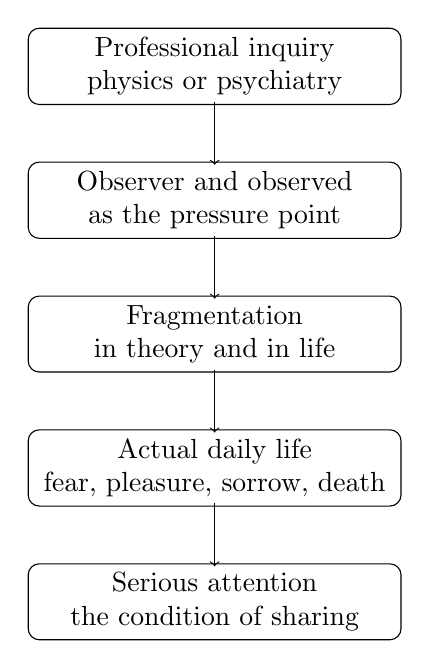
\begin{tikzpicture}[x=1cm,y=1cm]
\node[draw, rounded corners, align=center, text width=4.5cm] at (0,0) {Professional inquiry\\physics or psychiatry};
\node[draw, rounded corners, align=center, text width=4.5cm] at (0,-1.7) {Observer and observed\\as the pressure point};
\node[draw, rounded corners, align=center, text width=4.5cm] at (0,-3.4) {Fragmentation\\in theory and in life};
\node[draw, rounded corners, align=center, text width=4.5cm] at (0,-5.1) {Actual daily life\\fear, pleasure, sorrow, death};
\node[draw, rounded corners, align=center, text width=4.5cm] at (0,-6.8) {Serious attention\\the condition of sharing};
\draw[->] (0,-0.45) -- (0,-1.25);
\draw[->] (0,-2.15) -- (0,-2.95);
\draw[->] (0,-3.85) -- (0,-4.65);
\draw[->] (0,-5.55) -- (0,-6.35);
\end{tikzpicture}
\caption{A transcript-based map of the introductory movement. This is an editorial reconstruction, not a blackboard figure.}
\end{figure}

\section{Krishnamurti's Demand For Seriousness}

The interviewer then turns to Krishnamurti and asks how the viewer can best share in these dialogues. Krishnamurti's answer changes the level of the discussion. He does not begin by asking whether the viewer understands physics, psychiatry, or the history of Brockwood Park. He says it depends on how serious one is: how deeply one wants to go into these questions, which are, after all, one's life.

This is the decisive pivot of the lecture. The dialogue is not about abstract hypotheses. It is about actual daily life. Krishnamurti names the facts:
\begin{equation}
\mathcal{A}
=
\{\text{fear},\ \text{pleasure},\ \text{sorrow},\ \text{death},\ \text{the sacred}\}.
\end{equation}
Here \(\mathcal{A}\) stands for the field of actual inquiry. It is not a psychological taxonomy. It is a reminder that the conversation is not meant to float above life.

Krishnamurti's point can be stated as a proposition.

\begin{proposition}
In this dialogue, participation is not primarily agreement, belief, or interpretation. Participation requires seriousness, care, and attention to the actual facts of one's own life.
\end{proposition}

\begin{proof}
The transcript moves from the viewer's question, ``How can he gain the most from the experience?'' to Krishnamurti's answer that everything depends on seriousness. He immediately distinguishes the inquiry from theoretical abstraction and names actual daily life as the field. Therefore the condition of sharing is not technical knowledge alone, but the quality of attention brought to the facts under discussion.
\end{proof}

The word ``attention'' should not be softened into a technique. In the lecture it belongs with care and seriousness. One can share in the dialogue only if one is willing to let the inquiry concern fear, pleasure, sorrow, death, and the question of whether there is anything sacred in life. Without something real or true, Krishnamurti says, life has very little meaning.

\section{Summary}

This introductory lecture establishes the ground for the larger inquiry into happiness and transformation. Bohm brings the discipline of theoretical physics and the deeper questions of time, space, matter, causality, and the observer/observed relation. Shainberg brings the difficulty of psychiatry: fragmentation may be studied by theories that are themselves fragmented. Krishnamurti then turns the whole matter toward the viewer and the actual facts of daily life.

The chapter should therefore preserve three movements:
\begin{enumerate}
\item From physics to the observer and the observed.
\item From psychiatry to the problem of fragmentation.
\item From professional theory to serious attention to actual life.
\end{enumerate}
No validated lecture screenshots or blackboard equations support this chapter, so the displays and diagram used here are editorial aids. They should remain visibly subordinate to the transcript. The real spine of the lecture is not a formula but a demand: if we are to enter these dialogues, we must do so seriously, because the subject is our own life.